\documentclass{beamer}
\mode<presentation>
\usepackage{amsmath,amssymb,mathtools}
\usepackage{textcomp}
\usepackage{gensymb}
\usepackage{adjustbox}
\usepackage{subcaption}
\usepackage{enumitem}
\usepackage{multicol}
\usepackage{listings}
\usepackage{url}
\usepackage{graphicx} % <-- needed for images
\def\UrlBreaks{\do\/\do-}

\usetheme{Boadilla}
\usecolortheme{lily}
\setbeamertemplate{footline}{
  \leavevmode%
  \hbox{%
  \begin{beamercolorbox}[wd=\paperwidth,ht=2ex,dp=1ex,right]{author in head/foot}%
    \insertframenumber{} / \inserttotalframenumber\hspace*{2ex}
  \end{beamercolorbox}}%
  \vskip0pt%
}
\setbeamertemplate{navigation symbols}{}

\lstset{
  frame=single,
  breaklines=true,
  columns=fullflexible,
  basicstyle=\ttfamily\tiny   % tiny font so code fits
}

\numberwithin{equation}{section}

% ---- your macros ----
\providecommand{\nCr}[2]{\,^{#1}C_{#2}}
\providecommand{\nPr}[2]{\,^{#1}P_{#2}}
\providecommand{\mbf}{\mathbf}
\providecommand{\pr}[1]{\ensuremath{\Pr\left(#1\right)}}
\providecommand{\qfunc}[1]{\ensuremath{Q\left(#1\right)}}
\providecommand{\sbrak}[1]{\ensuremath{{}\left[#1\right]}}
\providecommand{\lsbrak}[1]{\ensuremath{{}\left[#1\right.}}
\providecommand{\rsbrak}[1]{\ensuremath{\left.#1\right]}}
\providecommand{\brak}[1]{\ensuremath{\left(#1\right)}}
\providecommand{\lbrak}[1]{\ensuremath{\left(#1\right.}}
\providecommand{\rbrak}[1]{\ensuremath{\left.#1\right)}}
\providecommand{\cbrak}[1]{\ensuremath{\left\{#1\right\}}}
\providecommand{\lcbrak}[1]{\ensuremath{\left\{#1\right.}}
\providecommand{\rcbrak}[1]{\ensuremath{\left.#1\right\}}}
\theoremstyle{remark}
\newtheorem{rem}{Remark}
\newcommand{\sgn}{\mathop{\mathrm{sgn}}}
\providecommand{\abs}[1]{\left\vert#1\right\vert}
\providecommand{\res}[1]{\Res\displaylimits_{#1}}
\providecommand{\norm}[1]{\lVert#1\rVert}
\providecommand{\mtx}[1]{\mathbf{#1}}
\providecommand{\mean}[1]{E\left[ #1 \right]}
\providecommand{\fourier}{\overset{\mathcal{F}}{ \rightleftharpoons}}
\providecommand{\system}{\overset{\mathcal{H}}{ \longleftrightarrow}}
\providecommand{\dec}[2]{\ensuremath{\overset{#1}{\underset{#2}{\gtrless}}}}
\newcommand{\myvec}[1]{\ensuremath{\begin{pmatrix}#1\end{pmatrix}}}
\let\vec\mathbf

\title{Matgeo Presentation - Problem 10.7.111}
\author{ee25btech11063 - Vejith}

\begin{document}


\frame{\titlepage}
\begin{frame}{Question}
Let the straight line $y = 2x$ touch a circle with center $(0, a)$, $a > 0$, and radius $r$ at a point $\vec{A_1}$. Let $\vec{B_1}$ be the point on the circle such that the line segment $\vec{A_1}\vec{B_1}$ is a diameter of the circle. Let $a + r = 5 + \sqrt{5}$. Match the following:\\

\begin{tabular}{ l l }

(A) $a$ equals & (1) \brak{-2,4}\\
(B)  r equals & 2. $\sqrt{5}$\\
(C)$\vec{A_1}$ equals  & (3)\brak{-2,6}\\
(D) $\vec{B_1}$ equals & (4) 5\\
	& (5) \brak{2,4}\\
\end{tabular}\\

The correct option is \hspace{7cm} \brak{2024}
\begin{enumerate}[label=\alph*)]

    \item A$- 4$, B$- 2$, C$- 1$, D$- 3$
    \item A$- 2$, B$- 4$, C$- 1$, D$- 3$
    \item A$- 4$, B$- 2$, C$- 5$, D$- 3$
    \item A$- 2$, B$- 4$, C$- 3$, D$- 5$
\end{enumerate}
\end{frame}

\begin{frame}{Solution}
    The equation of a Conic in Matrix form is
\begin{align}
\vec{x}^\top\vec{V}\vec{x} + 2\vec{u}^\top\vec{x} + f = 0
\end{align}
For the given circle. let $r$ be the radius of given circle 
\begin{align}
    \vec{V}=\begin{pmatrix}
        1 & 0\\
        0 & 1
    \end{pmatrix},\vec{u}=\myvec{0\\-a},f=a^2-r^2
\end{align}
Equation of Tangent is given by
\begin{align}
    \vec{n}^\top\vec{x}=c\\
    \implies \vec{n}=\myvec{2\\-1} ,c=0\\
    \implies \brak{2\hspace{0.5cm}-1}\myvec{x\\y}=0
\end{align}
\end{frame}

\begin{frame}{Solution}
The distance of point $\vec{P}$ to the line $\vec{n}^\top\vec{x}=c$ is given by
\begin{align}
    d=\frac{|\vec{n}^\top\vec{P}-c|}{\norm{\vec{n}}}\\
    \implies r = \frac{\left\lvert
\begin{pmatrix} 2 & 1 \end{pmatrix}
\begin{pmatrix} 0 \\ -a \end{pmatrix} - 0
\right\rvert}{\sqrt{5}}\\
\implies r=\frac{a}{\sqrt{5}}
\end{align}
\begin{align}
a + r = 5 + \sqrt{5}
\end{align}
substitute (8) in (9)
\begin{align}
\sqrt{5}r +r =5 +\sqrt{5}\\
    \implies r=\sqrt{5}\\
    \implies a=5
\end{align}
\end{frame}

\begin{frame}{Solution}
For a circle, the points of contact are
\begin{align}
    \vec{q_{j}}=\brak{\pm r \frac{\vec{n_j}}{\norm{\vec{n_j}}}-\vec{u}},j=1,2
\end{align}
let $\vec{A_1}$ be the point of contact
\begin{align}
    \vec{A_1}=\brak{-r \frac{\vec{n}}{\norm{\vec{n}}}-\vec{u}}\\
    =\brak{\frac{r}{\sqrt{5}}\myvec{2\\-1}-\myvec{0\\-a}} \hspace{0.5cm}\\ 
    \implies \vec{A_1}=\myvec{2\\4}
\end{align}
\end{frame}

\begin{frame}{Conclusion}
Given  $\vec{A_1}$ and $\vec{B_1}$ is the diameter of the circle 
\begin{align}
    \frac{\vec{A_1}+\vec{B_1}}{2}=\vec{u}\\
    \vec{B_1}=\brak{\vec{u} \hspace{0.5cm} \vec{A_1}}\myvec{2\\-1}\\
    \vec{B_1}=\myvec{-2\\6}
\end{align}
Answer is c) A$- 4$, B$- 2$, C$- 5$, D$- 3$
\end{frame}

\begin{frame}{Plot}
    \begin{figure}[h!]
    \centering
    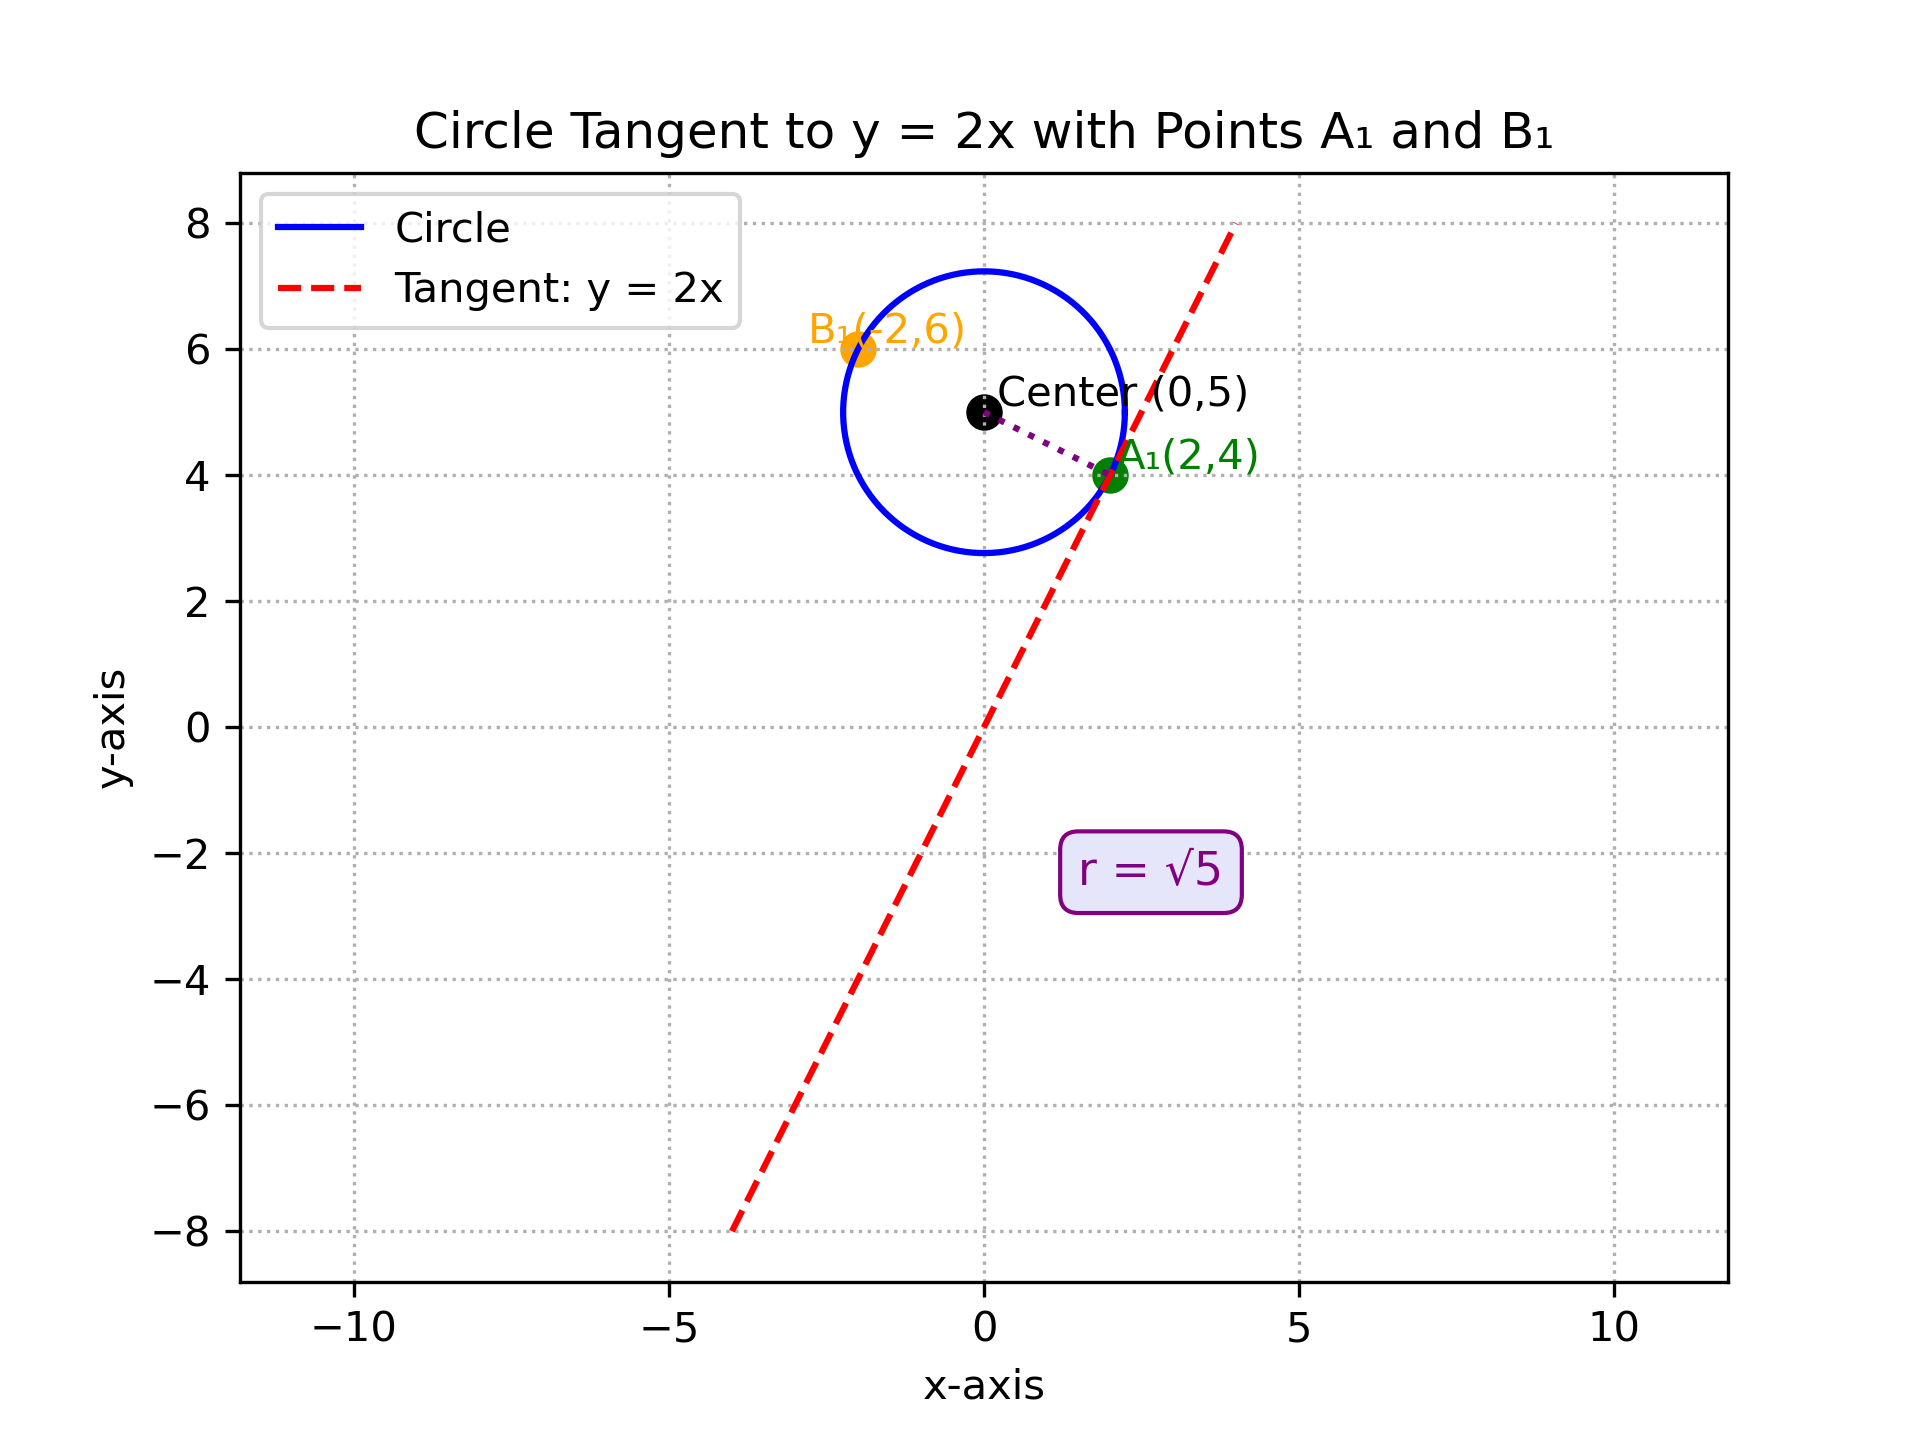
\includegraphics[width=0.8\columnwidth]{figs/01.png}
    \caption{}
    \label{fig:placeholder}
\end{figure}
\end{frame}

% --------- CODE APPENDIX ---------
\section*{Appendix: Code}

% C program
\begin{frame}[fragile]{C Code: circle.c}
\begin{lstlisting}[language=C]
#include <stdio.h>
#include <math.h>

int main() {
    FILE *fp;
    double a, r;
    double A1x, A1y, B1x, B1y;

    // Given relation: a + r = 5 + sqrt(5)
    // and r = a / sqrt(5)
    // So we solve for a and r
    a = 5;
    r = sqrt(5);

    // Coordinates of A1 (point of tangency)
    A1x = 2;
    A1y = 4;

    // Coordinates of B1 (diametrically opposite point)
    B1x = -2;
    B1y = 6;

    // Open file to write output
    fp = fopen("circle.dat", "w");
    if (fp == NULL) {
        printf("Error opening file!\n");
        return 1;
    }
\end{lstlisting}
\end{frame}

\begin{frame}[fragile]{C Code: circle.c}
\begin{lstlisting}[language=C]
    fprintf(fp, "Results of the circle problem:\n");
    fprintf(fp, "--------------------------------\n");
    fprintf(fp, "(A) a = %.2f\n", a);
    fprintf(fp, "(B) r = %.5f\n", r);
    fprintf(fp, "(C) A1 = (%.2f, %.2f)\n", A1x, A1y);
    fprintf(fp, "(D) B1 = (%.2f, %.2f)\n", B1x, B1y);
    fprintf(fp, "\nMatching options:\n(A)->(4), (B)->(2), (C)->(5), (D)->(3)\n");
    fprintf(fp, "Correct Option: (c)\n");

    fclose(fp);

    printf("Results written successfully to circle.dat\n");

    return 0;
}
\end{lstlisting}
\end{frame}

% Python plotting
\begin{frame}[fragile]{Python: plot.py}
\begin{lstlisting}[language=Python]
import matplotlib.pyplot as plt
import numpy as np
import math

# Given values
a = 5                  # y-coordinate of center
r = math.sqrt(5)       # radius
center = (0, a)
A1 = (2, 4)
B1 = (-2, 6)

# Generate circle
theta = np.linspace(0, 2 * np.pi, 400)
x_circle = r * np.cos(theta)
y_circle = a + r * np.sin(theta)

# Tangent line y = 2x
x_line = np.linspace(-4, 4, 200)
y_line = 2 * x_line

# Plot circle and tangent
plt.plot(x_circle, y_circle, label='Circle', color='blue')
plt.plot(x_line, y_line, color='red', linestyle='--', label='Tangent: y = 2x')

# Plot key points
plt.scatter(*center, color='black', s=60)
plt.scatter(*A1, color='green', s=60)
plt.scatter(*B1, color='orange', s=60)

# Draw radius line
plt.plot([center[0], A1[0]], [center[1], A1[1]], color='purple', linestyle=':')
\end{lstlisting}
\end{frame}

\begin{frame}[fragile]{Python: plot.py}
\begin{lstlisting}[language=Python]
plt.text(2.1, 4.1, "A₁(2,4)", color='green', fontsize=10)
plt.text(-2.8, 6.1, "B₁(-2,6)", color='orange', fontsize=10)
plt.text(0.2, 5.1, "Center (0,5)", color='black', fontsize=10)

# Box below tangent equation showing radius
plt.text(1.5, -2.5, "r = √5", fontsize=11, color='purple',
         bbox=dict(facecolor='lavender', edgecolor='purple', boxstyle='round,pad=0.4'))

# Make it neat
plt.axis('equal')
plt.grid(True, linestyle=':')
plt.xlabel('x-axis')
plt.ylabel('y-axis')
plt.title('Circle Tangent to y = 2x with Points A₁ and B₁')
plt.legend(loc='upper left')
plt.savefig('circle.png', dpi=300)
plt.show()

  \end{lstlisting}
\end{frame}
\end{document}
